\begin{frame}
	\frametitle{Pedosphäre - Böden}

	\begin{figure}
		\centering
		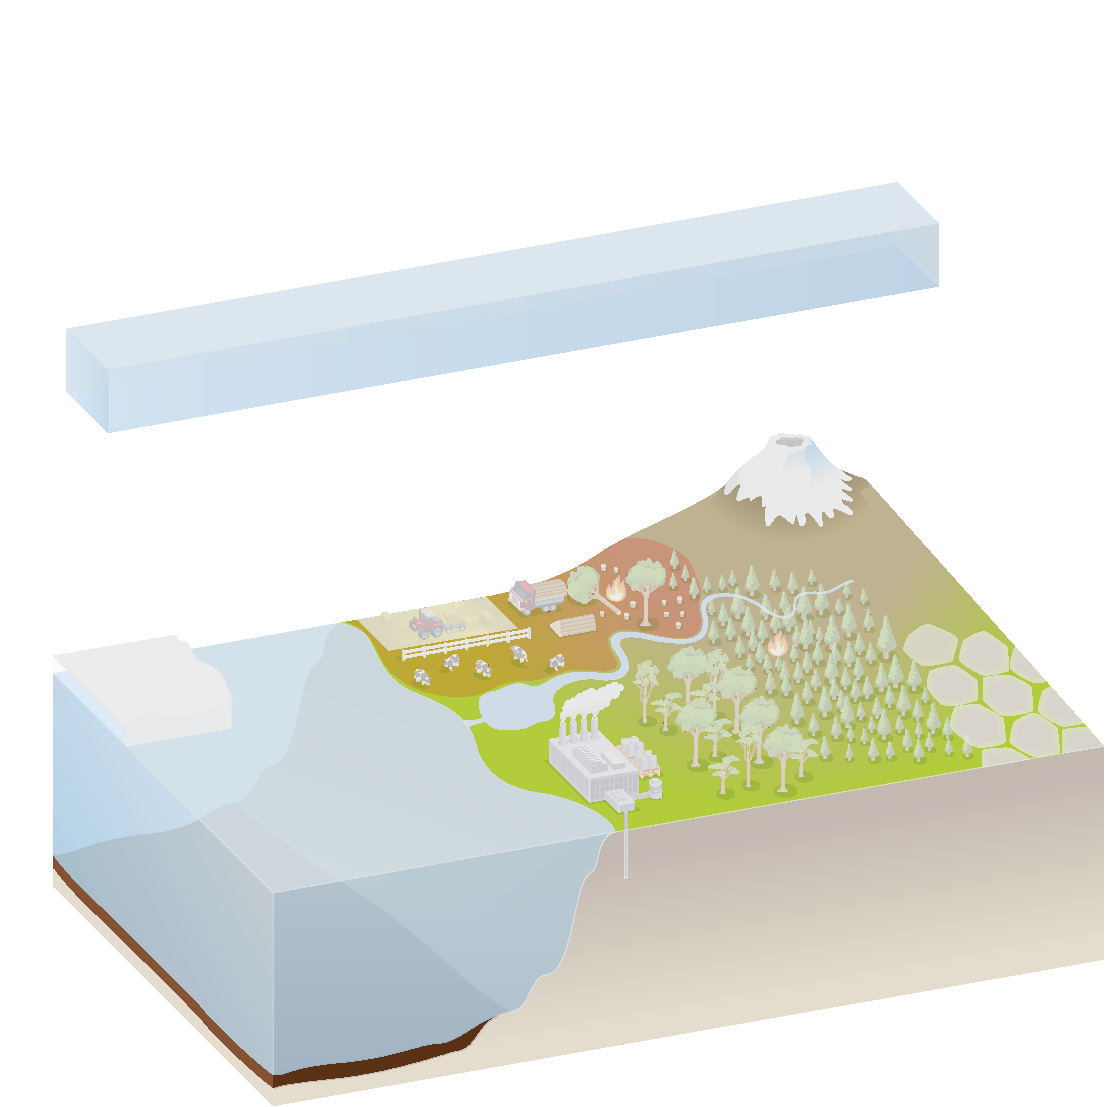
\includegraphics[trim={1cm 0cm 0cm 3cm}, clip, width=0.55\linewidth]{%
        bilder/climate_components/global_climate_components_pedosphere.pdf}
		\caption{Die Pedosphäre bezeichnet ist der Bereich der Erdoberfläche in dem sich Lithosphäre, Hydrosphäre, Atmosphäre und Biosphäre überschneiden.}
	\end{figure}

	\note{
		\begin{itemize}
			\item[] Boden
		\end{itemize}
	}
\end{frame}
